\subsection{The stations and their geographic context}
\label{sec:contexto-estaciones}

The MMA occupies a valley at about 500 m above sea level (a.s.l.), bounded to
the south and west by the Sierra Madre Oriental, to the east by Cerro de la
Silla and to the north by Cerro del Topo Chico and Sierra de las Mitras. The
15 SIMA stations are spread across this valley along an elevation gradient
from 334 m a.s.l., on the southeastern plain, to 702 m a.s.l., at the foot of
the mountains in the northwest (\cref{tab:estaciones}). Each station code
indicates its quadrant, and from it the stations are grouped into seven
zones that the models of \cref{sec:clasificacion_tecs} use as a categorical
predictor.

\begin{table}[pos=t]
  \centering
  \caption{SIMA stations, the zone to which each is assigned, and elevation.
    Coordinates in degrees and minutes; all north latitude and west
    longitude.}
  \label{tab:estaciones}
  \small
  \begin{tabular}{llrll}
    \toprule
    Code & Zone & m a.s.l. & Lat. & Long. \\
    \midrule
    \texttt{SE3}  & Southeast & 334 & 25°36' & 100°00'  \\
    \texttt{NE3}  & Northeast & 346 & 25°47' & 100°05' \\
    \texttt{SE2}  & Southeast & 387 & 25°39' & 100°06' \\
    \texttt{NE2}  & Northeast & 432 & 25°47' & 100°11' \\
    \texttt{NE}   & Northeast & 474 & 25°45' & 100°15' \\
    \texttt{SE}   & Southeast & 500 & 25°40' & 100°15' \\
    \texttt{NTE}  & North     & 503 & 25°48' & 100°20' \\
    \texttt{NTE2} & North     & 520 & 25°44' & 100°19' \\
    \texttt{SUR}  & South     & 555 & 25°37' & 100°16' \\
    \texttt{CE}   & Center    & 562 & 25°41' & 100°20' \\
    \texttt{NO}   & Northwest & 568 & 25°46' & 100°22' \\
    \texttt{NO3}  & Northwest & 607 & 25°46' & 100°28' \\
    \texttt{SO2}  & Southwest & 636 & 25°40' & 100°25' \\
    \texttt{SO}   & Southwest & 674 & 25°41' & 100°27' \\
    \texttt{NO2}  & Northwest & 702 & 25°48' & 100°35' \\
    \bottomrule
  \end{tabular}
\end{table}

Three geographic factors shape the measurements. The first is wind: the
median zonal wind component is negative (\cref{tab:cuartiles-iqr}), that is,
the prevailing wind enters from the east and carries the precursors emitted
in the center and east of the city toward the west, where the mountains
block their exit. The second is elevation, which covaries with distance to
\ce{NOx} sources and with land use: the correlation between a station's
elevation and its exceedance rate is 0.827 across the 15 stations
(\cref{fig:elevacion-excedencia}). The third is the orographic enclosure
already described in \cref{sec:objetivo}, which prevents vertical and
horizontal dispersion during episodes of high pressure and weak wind. The
result is a west--east ordering that is stable across the four seasons: the
Northwest and Southwest have the highest exceedance rates (43.3\,\% and
42.1\,\%) and the Northeast the lowest (19.5\,\%).

\begin{figure}[pos=t]
  \centering
  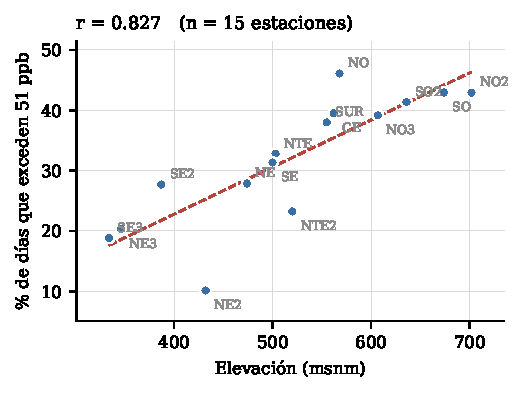
\includegraphics[width=\linewidth]{elevacion_vs_excedencia.pdf}
  \caption{MDA8 exceedance rate at 51 ppb versus the elevation of each
    station, 2021--2025. With $n=15$ and correlated neighboring stations,
    the line describes an association, not an effect of altitude.}
  \label{fig:elevacion-excedencia}
\end{figure}

Two considerations limit comparability across stations. \texttt{NO3} has
operated only since December 2022, so its window is shorter; and no station
measures volatile organic compounds, the second ozone precursor, which
restricts any chemical interpretation to nitrogen oxides, with \ce{CO} as a proxy.
